% !TeX spellcheck = <none>
\documentclass[11pt,a4paper,english,oneside]{book}

\usepackage{etex} %Because of many packages --> Extended TeX.
\usepackage[left=1in, right=1in]{geometry} %Helps to structure the paper layout.
\usepackage[Lenny]{fncychap} %Design of the thesis.
\usepackage[utf8]{inputenc} %Due to vowels.
\usepackage[T1]{fontenc}
\usepackage[ngerman]{babel} %Define the language style.

% german language for appendix header
\addto\captionsngerman{\let\appendixtocname\appendixname%
	\let\appendixpagename\appendixname}

% Setup glossary and acronyms
\usepackage[acronym,toc,nopostdot]{glossaries}
\loadglsentries{glossar-terms}
\glsenablehyper
\makeglossaries

% Include external pdf
\usepackage{pdfpages}

% set single pages to landscape
\usepackage{lscape}

\usepackage{dsfont} %Nice style for the indicator function.
\usepackage{fancyhdr} %To customize the headers and footers.
\usepackage{booktabs} %In case you need \cmidrule or \addlinespace in tables.
\usepackage[hang,bottom,stable,multiple]{footmisc} %Style of footnotes.
\usepackage{appendix} %For the \appendixpage command.
%Load some mathematical packages.
\usepackage{amsmath}
\usepackage{amsfonts}
\usepackage{amsmath}
\usepackage{amssymb}
\usepackage{mathtools}
\usepackage[
backend=biber,
style=numeric,
sortlocale=de_CH,
natbib=true,
doi=true,
eprint=false
]{biblatex}  % Bibliography
\addbibresource{References.bib}
\usepackage{etoolbox} %To remove the page number on \appendixpage.
\usepackage{amsthm} %For theorems, definitions etc.
\usepackage{thmtools} %For theorems, definitions etc.
\usepackage{setspace} %Use double spacing.
\usepackage{lipsum} %For the \lipsum command to generate a text.
\usepackage{datetime} %For the specification of the date.
%\usepackage{tocloft} %The ToC, LoF and LoT each appear not necessarily on a new page.
\usepackage{graphicx,listings,xcolor,textcomp} %For the graphics, listings etc.
\usepackage{mcode} %To implement a Matlab code.
\usepackage[margin=10pt, font=small, labelfont=bf, labelsep=endash]{caption} %Customize the captions.
\usepackage{chngcntr} %To use counterwithout.
\usepackage{epstopdf} %For inserting .eps files into the document.
\usepackage{hyperref} %Must be loaded at the end.
\usepackage{xparse} %Load for \NewDocumentCommand command.
\usepackage{cleveref} %For the command \cref, load after hyperref.
\usepackage{arydshln} %Due to the capability to draw horizontal/vertical dash-lines.
\usepackage{array,hhline} %To create tables and matrices.
\usepackage{rotating} %To rotate a table.
\usepackage{tabularx} %An extended version of tabular.
\renewcommand{\arraystretch}{1.25}




%Setup of the reference links.
\hypersetup{
	colorlinks=true,
	linkcolor=cyan,
	anchorcolor=black,
	citecolor=cyan,
	filecolor=cyan,
	urlcolor=cyan,
	runcolor=cyan,
	menucolor=black
}


%Define some reasonable margins.
\setlength{\textwidth}{6.6in}
\setlength{\textheight}{8.8in}
\setlength{\topmargin}{-0.1in}
\setlength{\oddsidemargin}{0in}
\setlength{\parskip}{1mm}


\allowdisplaybreaks[1] %Page breaks of equations are allowed, but avoided if possible. 2-4 more relaxed.

%New command for the HSR logo.
\newcommand*{\plogo}{
\includegraphics{logo_hsr.pdf}}

%New command for the differential d to have an ordinary d.
\makeatletter
\newcommand{\ud}{\mathrm{d}}
\makeatother

%Remove page number on \appendixpage. Use the package 'etoolbox'.
\makeatletter
\patchcmd{\@chap@pppage}{\thispagestyle{plain}}{\thispagestyle{empty}}{}{}
\makeatother

%Declare Definitions, Theorems etc.
%%%%%%%%%%%%%%%%%%%%%%%%%%%%%%%%%%%%%%%%%%%%%%%%%%%%%%%%%%%%%%%%%%%%%%%%%%%%%%%%%%%%%%%%%%%%%%%%%%%%%%%%%%%%%%%%%%%
\declaretheorem[style=definition,qed=$\blacktriangleleft$, numberwithin=chapter]{remark} %additional options; numberwithin=,..., see 'Thmtools' Users’ Guide
\declaretheorem[style=definition,qed=$\triangle$,numberwithin=chapter]{definition}
\newtheorem{ass}{Assumption}[chapter]
\newtheorem{prop}{Proposition}[chapter]
\newtheorem{lemma}{Lemma}[chapter]
\declaretheorem[style=definition,qed=$\perp$,numberwithin=chapter]{example}
\newtheorem{theorem}{Theorem}[chapter]
\newtheorem{coroll}{Corollary}[chapter]
%%%%%%%%%%%%%%%%%%%%%%%%%%%%%%%%%%%%%%%%%%%%%%%%%%%%%%%%%%%%%%%%%%%%%%%%%%%%%%%%%%%%%%%%%%%%%%%%%%%%%%%%%%%%%%%%%%%

%Readjust the numbering.
\counterwithout{footnote}{chapter}
\numberwithin{equation}{chapter}


%\setlength{\parindent}{0cm} %Uncomment this if you don't want to have indents.

%----------------------------------------------------------------------------------------
%	TITLE PAGE
%----------------------------------------------------------------------------------------
\newcommand*{\titleGP}{\begingroup %Create the command for including the title page in the document.
	\centering %Center all text.
	\vspace*{\baselineskip} %White space at the top of the page.
	\plogo\\[2\baselineskip] %University Logo.
	\rule{\textwidth}{1.6pt}\vspace*{-\baselineskip}\vspace*{2pt} %Thick horizontal line.
	\rule{\textwidth}{0.4pt}\\[\baselineskip] %Thin horizontal line.
	{\LARGE Graphs-Visualization-Service }\\[0.2\baselineskip] %Title.
	\rule{\textwidth}{0.4pt}\vspace*{-\baselineskip}\vspace{3.2pt} %Thin horizontal line.
	\rule{\textwidth}{1.6pt}\\[2\baselineskip] %Thick horizontal line.
	\scshape %Small caps.
	\large Studienarbeit \\[2\baselineskip]
	Abteilung Informatik \par
	Hochschule für Technik Rapperswil
	\vspace*{2\baselineskip}
	
	
	Autoren\\
	{\Large  Michael Wieland  \\ [5pt]}
	
	{\Large Murièle Trentini \\ [5pt]}
	
	\vspace*{2\baselineskip}
	Betreuer\\
	{\Large Thomas Letsch  \\[5pt]
		\small Dozent für Informatik an der \\[5pt]Hochschule für Technik Rapperswil\par}
	\vspace*{2\baselineskip}
	
	Auditor\\
	{\Large [ Name ] \\[5pt]}
	\vspace*{2\baselineskip}
	
	\vfill
	{\scshape Zeitraum: 18.09.2017 - 22.12.2017} \\[0.3\baselineskip]
	\endgroup}


%Special header and footer style for the executive summary and Task Assignment section.
\fancypagestyle{firststyle}{%
	\fancyhf{}%
	\renewcommand{\headrulewidth}{0pt}
	\fancyfoot[C]{\thepage}}

%Customize headers and footers.
\pagestyle{fancy}
\fancyhead[R]{\thepage}
\fancyhead[L]{\rightmark}
\fancyfoot[L]{[Murièle Trentini | Michael Wieland ]}
\fancyfoot[C]{}
\fancyfoot[R]{[ GVS ]}

%Define the signature line with dots.
\NewDocumentCommand \dotbox {o O{.5\linewidth} m O{3ex} O{\linewidth}}
{
	\begin{minipage}{7cm}
		\makebox[7cm][l]{\,.\dotfill}
		\\
		\makebox[7cm][l]{\,#3}
	\end{minipage}
}

\begin{document}
	\thispagestyle{empty}
	\titleGP
	\newpage
	\doublespacing
	\setcounter{page}{1}
	\pagenumbering{Roman}
	\section*{Abstract}
	\thispagestyle{firststyle}
	
	
	\newpage
	
	\section*{Management Summary}
	\thispagestyle{firststyle}
	
	\subsection*{Ausgangslage}
	
	\subsection*{Vorgehen, Technologien}
	
	\subsection*{Ergebnisse}
	
	\subsection*{Ausblick}
	
	\newpage
	
	\section*{Danksagungen}
	\thispagestyle{firststyle}
	
	Wir danken folgenden Personen für Ihre Unterstützung während der Studienarbeit:
	
	\begin{itemize}
		\item Thomas Letsch für die Betreuung unserer Studienarbeit.
		\item Jessica Martin für die technische Unterstützung beim Logo Design.
	\end{itemize}

	{
		\hypersetup{linkcolor=black}
		\tableofcontents
	}
	
	\newpage
	\pagenumbering{arabic}
	% \part{[ Part title ]}
	\chapter{Anforderungsanalyse}
	
	\begin{table}[h!]
		\centering
		\begin{tabularx}{\linewidth}{l l X l}
			\toprule 
			Datum & Version & Änderungen & Autor \\
			\midrule
			28.09.17 & 1.0 & Grundgerüst erstellt & mwieland \\
			17.10.17 & 1.1 & Sequenzdiagramme eingefügt & mtrentini \\
			18.10.17 & 1.2 & Ausgangslage und Stakeholder eingefügt & mwieland \\
			19.10.17 & 1.3 & Erkennisse: Stärken, Schwächen, Schlüsse beschrieben & mwieland \\
			\bottomrule 
		\end{tabularx} 
		\caption{Versionshistory Anfoderungsanalyse} 
	\end{table}
	
	\section{Ausgangslage \& Problembeschreibung}
	Die Software \gls{gvs} unterstützt Studenten beim Erlernen der Datenstrukturen Tree und Graph, sowie der darauf anwendbaren Algorithmen. Der wichtigste Aspekt ist dabei die Visualisierung der Arbeitsweise von Datenstrukturen und Algorithmen. So zeigt die Software zum Beispiel den schrittweisen Aufbau eines Baumes oder den Ablauf des Path Finding Algorithmus ''Dijkstra''. \\
	Die Software wurde 2005 bereits im Rahmen einer Bachelorarbeit umgesetzt. Der in die Jahre gekommene GVS 1.0 soll nun in einem Major-Upgrade aktualisiert werden.
	
	\subsection{Mehrwert}
	\gls{gvs} wird nun auf den neusten der Technik gebracht und profitiert von neueren Java Features wie Generics und Lambdas sowie einer klaren und erweiterbaren Schichtenarchitektur. 
	Der Endbenutzer bemerkt nur eine modernes und ansprechendes User Interface. Die Funktionalität soll beibehalten werden. 

	
	\section{Anforderungen}
	Die Anforderungen wurden massgeblich aus der offiziellen Aufgabenstellung entnommen. (siehe Anhang \ref{aufgabenstellung})
	
	\begin{enumerate}
		\item Serverseitig muss das UI Framework Swing durch den offiziellen Nachfolger \gls{javafx} ersetzt werden.
		\item Clientseitig muss die Java und .NET Library um Generics erweitert werden. 
		\item Punktuell müssen Verbesserungen vorgenommen werden.
	\end{enumerate}

	Eine genauere Definition der dritten Anforderung, hat das Projektteam zusammen mit dem Betreuer, Herr Letsch, festgelegt und ist dem Abschnitt Refactroing Ablauf (\ref{ssec:ablauf}) zu entnehmen.
	
	\section{Domainanalyse}
	In der Domainanalyse hat sich das Projektteam einen Überblick über den aktuellen Stand von GVS 1.0 verschafft. Die dabei gewonnen Erkenntnisse sind in die Designspezifikation eingeflossen.
	
	\subsection{Stakeholder}
	Aus den Anforderungen für GVS 1.0 kristallisieren sich drei relevante Stakeholder heraus. Während der Realisierung des UI sollen die Bedürfnisse der Studenten berücksichtigt werden. Zusätzlich muss das Projektteam den Ansprüchen zukünftiger Entwickler an eine erweiterbare Architektur gerecht werden.
	\begin{table}[h!]
		\centering
		\begin{tabularx}{\linewidth}{l l X X}
			\toprule 
			\# & Rolle & Ziel/Intention & Erwartungshaltung \\
			\midrule
			1 & Student & Möchte GVS unkompliziert installieren und benutzen können. & Möchte den zu visualisierenden Graphen/Tree ansprechend dargestellt bekommen. Ihm ist der Lerneffekt wichtig.  \\
			2 & Entwickler & Möchte GVS einfach erweitern können. & Sucht nach bekannten Software Pattern und klaren Software Schichten.  \\			
			3 & Dozent & Möchte GVS in seinem Unterricht einsetzen. & Erwartet eine intuitive Integration von GVS in bestehende Übungsaufgaben. \\
			\bottomrule 
		\end{tabularx} 
		\caption{Relevante Stakeholder} 
	\end{table}

	\subsection{Aktoren} \label{ssec:actors}
	Das System wird von zwei Aktoren beeinflusst
	
	\subsubsection{GVS User} \label{sssec:actor-user}
	Der User interagiert mit dem GVS Server über das User Interface. Er die aktuelle Session auf das Filesystem speichern oder eine Session von dort laden. Wenn ein Graph visualisiert ist, kann er die Koordinaten der Vertices neu berechnen lassen.
	
	\subsubsection{GVS Client Lib} \label{sssec:actor-lib}
	Die Client Lib wird in das Software Projekt des GVS User eingebunden. Sie sendet in \gls{xml} beschriebene Datenstrukturen über eine Socket Verbindung an den GVS Server.
	
	\subsection{Systemübersicht}
	Der Aktor \textit{User} (\ref{sssec:actor-user}) interagiert mit dem GVS System über den Presentation Layer. Beispielsweise fliesst beim Laden einer Session der Dataflow bis ins Access Layer, wo die Applikation mit dem FileSystem interagiert.
	Über den Access Layers verbindet sich der Aktor \textit{GVS Client Lib} (\ref{sssec:actor-lib}) mit dem System und sendet Daten, welche auf dem Presentation Layer angezeit werden.
	
	\begin{figure}[h!]
		\centering
		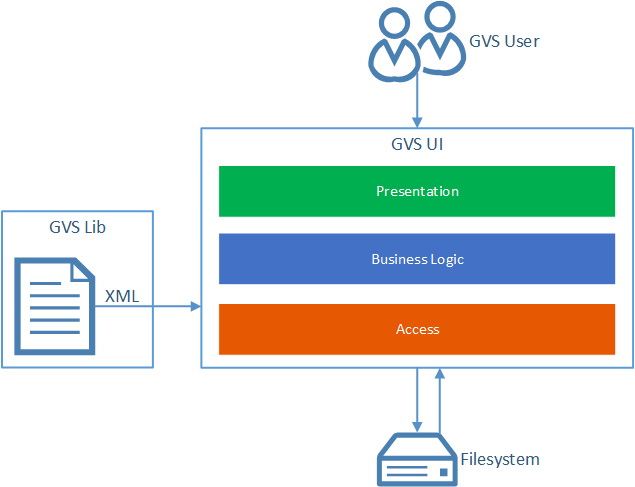
\includegraphics[width=0.7\linewidth]{assets/images/system_overview}
		\caption{Systemübersicht}
		\label{fig:gvs-systemuebersicht}
	\end{figure}
	
	\subsection{Klassendiagramm} \label{ssec:klassendiagramm-1}
	Das Klassendiagramm gab dem Projektteam eine gute Übersicht über die Struktur des GVS 1.0. Die Klassen wurden so organisiert, dass sie einer der drei Schichten ''Presentation'', ''Business'' und ''Access'' zugewiesen sind. Die aus der Analyse gezogenen Erkenntnisse sind im Abschnitt \ref{sec:erkenntnisse} genauer beschrieben.
	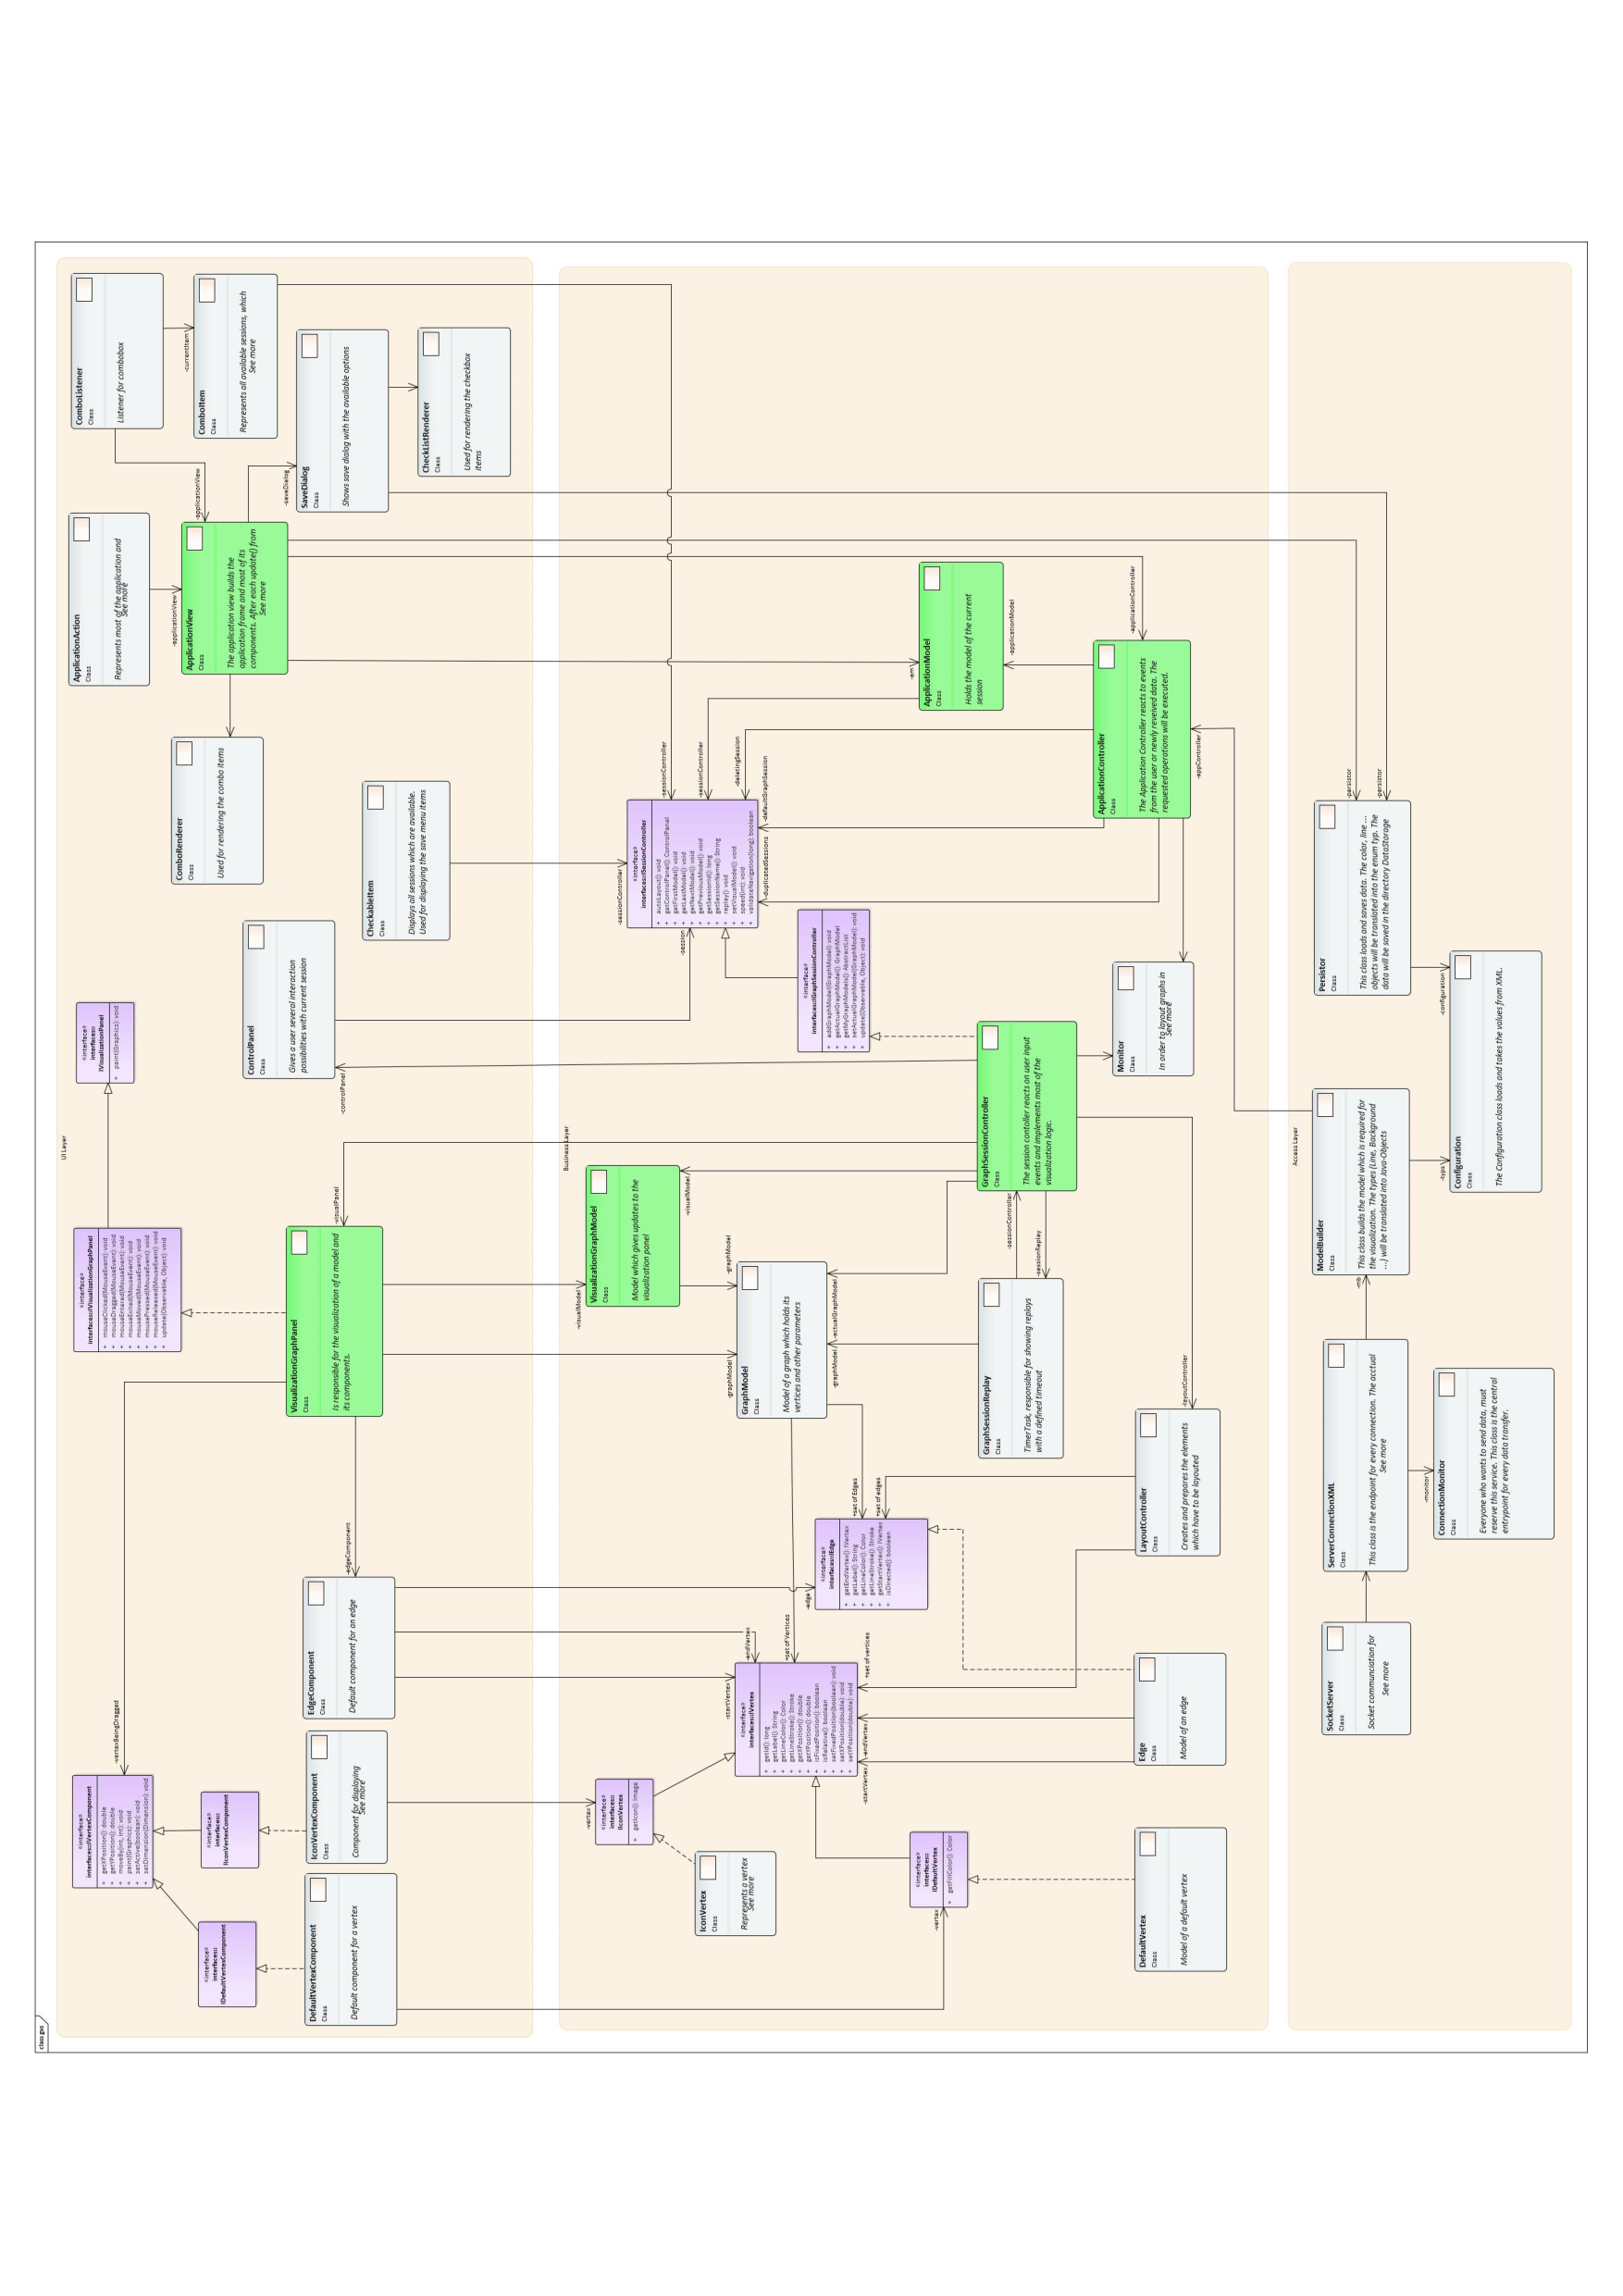
\includepdf[fitpaper]{assets/pdf/gvs1-0.pdf}
	
	\subsection{Sequenzdiagramme}
	Zum besseren Verständnis von GVS 1.0 hat das Projektteam die wichtigsten Systemabläufe analysiert und als Sequenzdiagramme aufgezeichnet.
	
	\subsubsection{Verbindungsaufbau}
	Dieses Sequenzdiagramm zeigt den Verbindungsaufbau über den \textit{SocketServer} beim starten der Applikation. Der Start einer \textit{SeverConnectionXML} führt zu einem Locking mit Hilfe des \textit{ConnectionMonitors}. Dieses Locking verhindert, dass mehr als ein Client gleichzeitig mit einem Server kommuniziert. Nach dem Empfangen der Daten aus dem Socket, erstellt der \textit{ModelBuilder} einen Graphen oder Tree als Domain-Objekt. Dieser Ablauf ist auf dem Sequenzdiagramm \textbf{ModelBuilder} (siehe \ref{sssec:modelbuilder}) ersichtlich.
	\begin{figure}[h!]
		\centering
		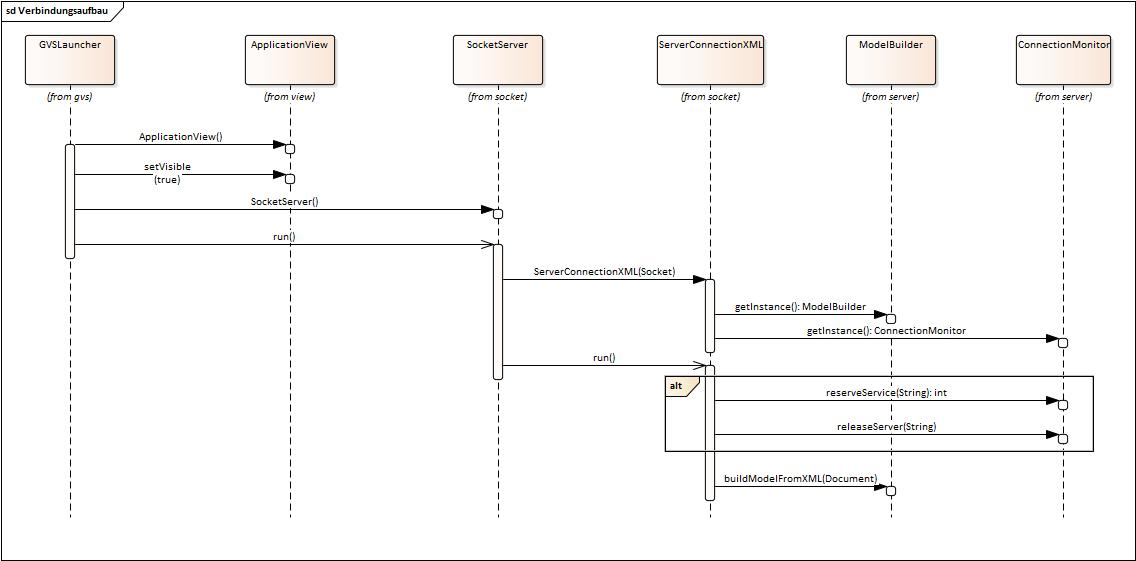
\includegraphics[width=\linewidth]{assets/images/verbindungsaufbau}
		\caption{Sequenzdiagramm: Verbindungsaufbau}
		\label{fig:sd-verbindungsaufbau}
	\end{figure}

	\subsubsection{ModelBuilder} 	\label{sssec:modelbuilder}
	Der \textit{ModelBuilder} parsed aus den empfangenen \gls{xml} Dokumenten das entsprechende Domain-Objekt. Dabei wird zwischen Graphen und Trees unterschieden. Nach Fertigstellung des Parse-Vorgangs, wird das Model an den entsprechenden \textit{SessionController} übergeben. Der weitere Ablauf befindet sich im separaten Sequenzdiagramm \textbf{GraphSessionController} (siehe \ref{sssec:sessioncontroller})
	\begin{figure}[h!]
		\centering
		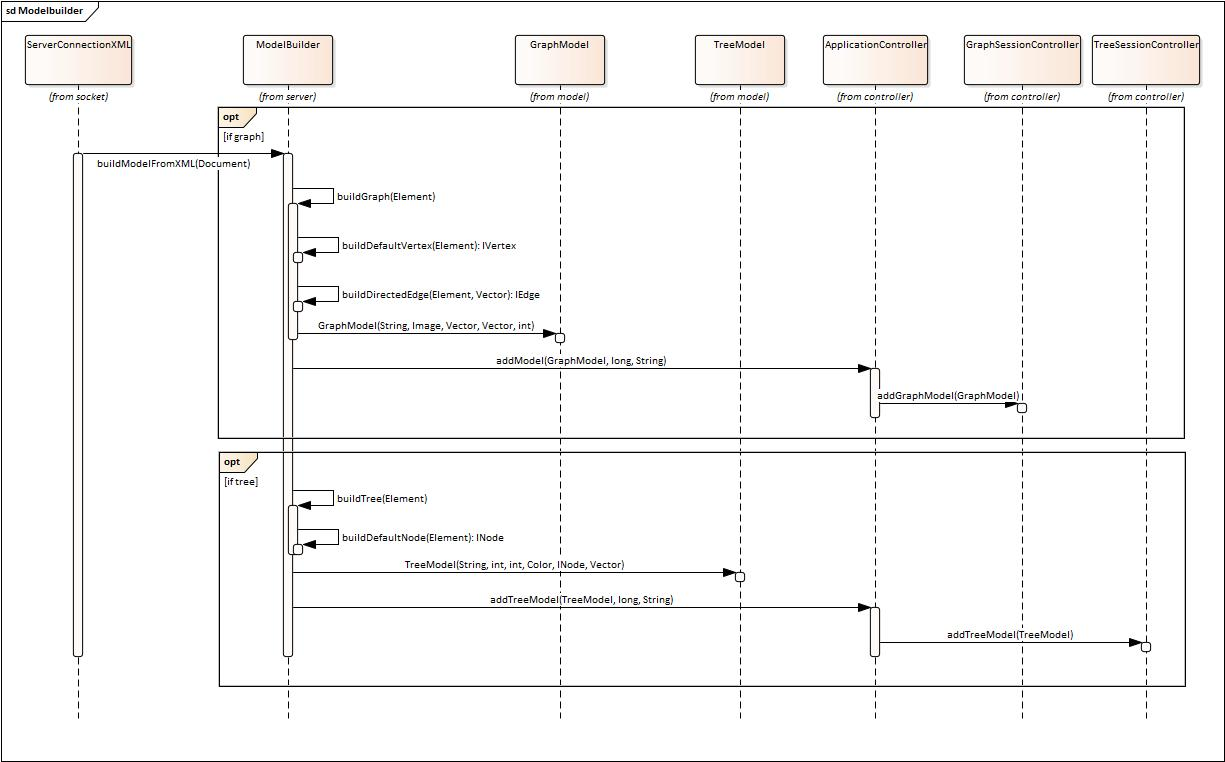
\includegraphics[width=\linewidth]{assets/images/modelbuilder}
		\caption{Sequenzdiagramm: ModelBuilder}
		\label{fig:sd-modelbuilder}
	\end{figure}

	\subsubsection{ApplicationView: Load \& Save Session} \label{sssec:appView}
	Wenn ein User eine Session lädt, wird das entsprechende \gls{xml} vom \textit{Persistor} geparsed. Dieser erstellt je nach Bedarf einen Vector aus Graphs oder Trees. Dieser Vector wird an den \textit{SessionController} übergeben. Der Ablauf innerhalb des \textit{SessionController}s ist im separaten Sequenzdiagramm \textbf{GraphSessionController} (siehe \ref{sssec:sessioncontroller}) dargestellt. \\
	Nachdem die Session erstellt wurde, wird die \textit{ApplicationView} per Observer-Beziehung (siehe Glossar: \gls{observer}) notifiziert. Sie stellt darauf die neue Session im UI dar.\\
	Auffällig an der Klasse \textit{ApplicationView} ist, dass sie im Constructor einen \textit{Persistor} instanziert. Diese Instanz wird jedoch nicht direkt in der ApplicationView verwendet, sondern wird als Argument an den \textit{ApplicationController} geschickt, welcher dann mit dem Persistor Sessions speichert und lädt. In der Analyse des Projektteams ist unklar geblieben, wieso die Instanzierung des \textit{Persistor}s nicht direkt im \textit{ApplicationController} passiert.
	\begin{figure}[h!]
		\centering
		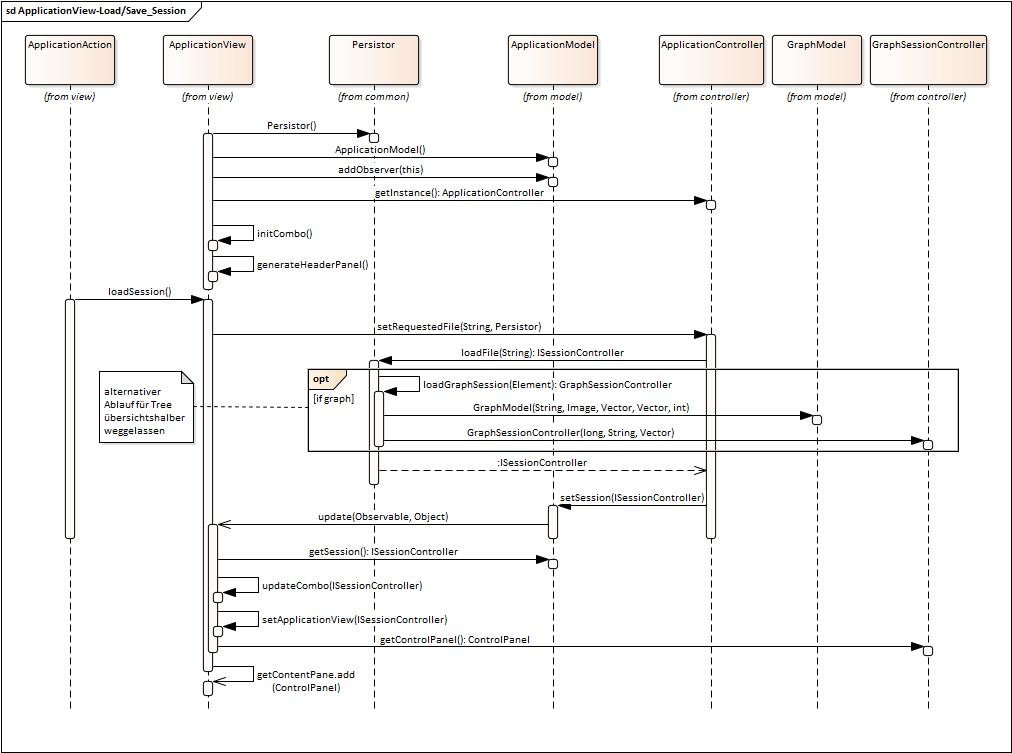
\includegraphics[width=\linewidth]{assets/images/application_view}
		\caption{Sequenzdiagramm: ApplicationView}
		\label{fig:sd-applicationview}
	\end{figure}

	\subsubsection{GraphSessionController} \label{sssec:sessioncontroller}
	Der \textit{GraphSessionController} wird vom \textit{ModelBuilder} und vom \textit{Persistor} angestossen, wenn ein oder mehrere neue Graphen geparsed wurden. Der \textit{GraphSessionController} ist dafür zuständig diese Graphen in eine neue oder bestehende Session einzufügen. Dabei unterscheidet sich der Programmablauf kaum. Übersichtshalber ist nur der Fall ''ein einzelner neuer Graph wurde empfangen'' abgebildet.\\
	Für Graphen die keine fix positionierte Vertices haben, wird in einem weiteren Schritt der \textit{LayoutController} aufgerufen. Dieser steuert die Funktionalität der Physics-Engine. Die Physics-Engine berechnet die Koordinaten von Vertices mittels anziehenden und abstossenden Kräften. (siehe \gls{forcedirecteddrawing}) Der \textit{GraphSessionController} wird  per Observer-Beziehung (siehe Glossar: \gls{observer}) informiert, sobald die Physics-Engine die Berechnung der Positionen abgeschlossen hat.\\
	Der \textit{GraphSessionController} setzt den neuen Graphen als aktuellen Graphen auf dem \textit{VisualizationGraphModel}. Dieses informiert per Observer-Beziehung (siehe Glossar: \gls{observer}) das \textit{VisualiztionGraphPanel}, welches die für die Darstellung benötigten Vertex und Edge Komponenten erstellt.
	\begin{figure}[h!]
		\centering
		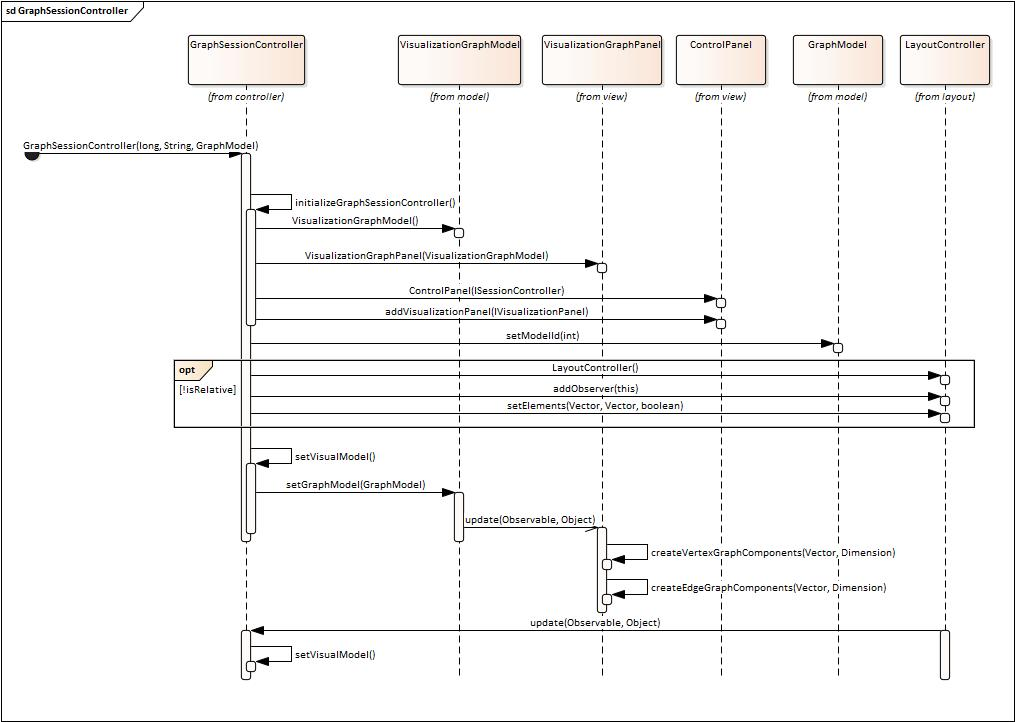
\includegraphics[width=\linewidth]{assets/images/graph_session_controller}
		\caption{Sequenzdiagramm: GraphSessionController}
		\label{fig:sd-graphsessioncontroller}
	\end{figure}
	
	\section{Erkenntnisse} \label{sec:erkenntnisse}
	Aus der Analysephase konnten wertvolle Erkenntnisse für das weitere Vorgehen gewonnen werden.
	
	\subsection{Stärken}
	Der GVS 1.0 weisst folgende Stärken auf:
	
	\subsubsection{Trennung Socket / Visualization}
	Die angedachte Trennung zwischen Server und Visualisierung der Daten widerspiegelt sich klar im vorliegenden Code.
	
	\subsubsection{Layering}
	Die meisten Klassen konnten bei der Analyse eindeutig einem Layer zugewiesen werden. Dies zeigt, dass die geplante Architektur mehrheitlich umgesetzt wurde.
		
	\subsection{Schwächen}
	Der GVS 1.0 weisst folgende Schwächen auf:
	
	\subsubsection{Swing/AWT Imports im Business Layer} 
	Im Business Layer wurden diverse Imports der UI Frameworks \gls{swing} rsp. \gls{awt} gefunden. Dies erschwert einen Austausch des eingesetzten UI Frameworks.
	
	\subsubsection{Tangles} Zwischen dem Presentation und Business Layer existieren \gls{tangle}s. Dies verhindert einen einfachen Austausch des Presentation Layers. 
	
	\subsubsection{Magic Numbers} Viele Konstanten wurden ungenügend beschrieben. Der Zweck von vielen Zahlen ist daher nur schwer nachvollziehbar.
	
	\subsubsection{Namenskonvention}
	Eine Prüfung der Namenskonvention wurde offenbar nicht durchgeführt. Zum Beispiel sind veränderbare Variablen in Grossbuchstaben geschrieben, was normalerweise auf eine Konstante hindeutet.
	
	\subsubsection{Temporary Fields}
	Viele Klassen arbeiten stark mit Klassenvariablen die in diversen Methoden gesetzt und gelesen werden. Zusätzlich werden diese auch von lokalen Variablen überdeckt. Dies erschwert es, dem Programmfluss folgen zu können.
	
	\subsubsection{Duplicated Code}
	Klassen wie der \textit{ModelBuilder} und \textit{Persistor} übernehmen sehr ähnliche Aufgaben.
	
	\subsubsection{Long Classes}
	Einige Klassen überschreiten die Obergrenze von 250 Zeilen Code/Klasse. Dies hebt den Verdacht, dass die Klassen mehr als eine Aufgabe erledigen und somit das ''Single Responsibility Principle'' verletzen.
	
	\subsubsection{Keine Unit Tests} Im Projekt wurden keine Unit Tests geschrieben. Der Grund dafür ist vermutlich, dass JUnit zum Entwicklungszeitpunkt noch sehr jung war.
	
	\subsubsection{JavaDoc}
	Das Verhalten von Klassen ist nicht durchgehend dokumentiert.  Ebenfalls fehlt es bei einigen Kommentaren an Aussagekraft.	
		
	\subsection{Schlüsse}
	Aus den gewonnen Erkenntnissen hat das Projektteam Metriken eingeführt, damit der neue Code auf die Einhaltung von Konventionen geprüft werden kann. Ebenfalls wurden vor dem Start der Realisierung erste Refactorings durchgeführt, um den alten Code an die neuen Metriken anzugleichen.

		
	\chapter{Designspezifikation}
	
	\begin{table}[h!]
		\centering
		\begin{tabularx}{\linewidth}{l l X l}
			\toprule 
			Datum & Version & Änderungen & Autor \\
			\midrule
			13.10.17 & 1.0 & MVVM Konzept geschrieben & mwieland \\
			19.10.17 & 1.1 & Refactoring Konzept erstellt & mtrentini \\
			\bottomrule 
		\end{tabularx} 
		\caption{Versionshistory Designspezifikation} 
	\end{table}
	
	\section{Klassendiagramm} \label{sec:class-diagram}
	Das neue Klassendiagramm orientiert sich stark an die Vorgängerversion des GVS 1.0. (Siehe \ref{ssec:klassendiagramm-1}). Mit dem Ziel möglichst viel Code wiederzuverwenden, wurde der Access und Business Layer mehrheitlich beibehalten. Der Presentation wurde vollständig durch die neu eingeführte \gls{mvvm} Struktur ersetzt. (Siehe \ref{sssec:mvvm})
	
	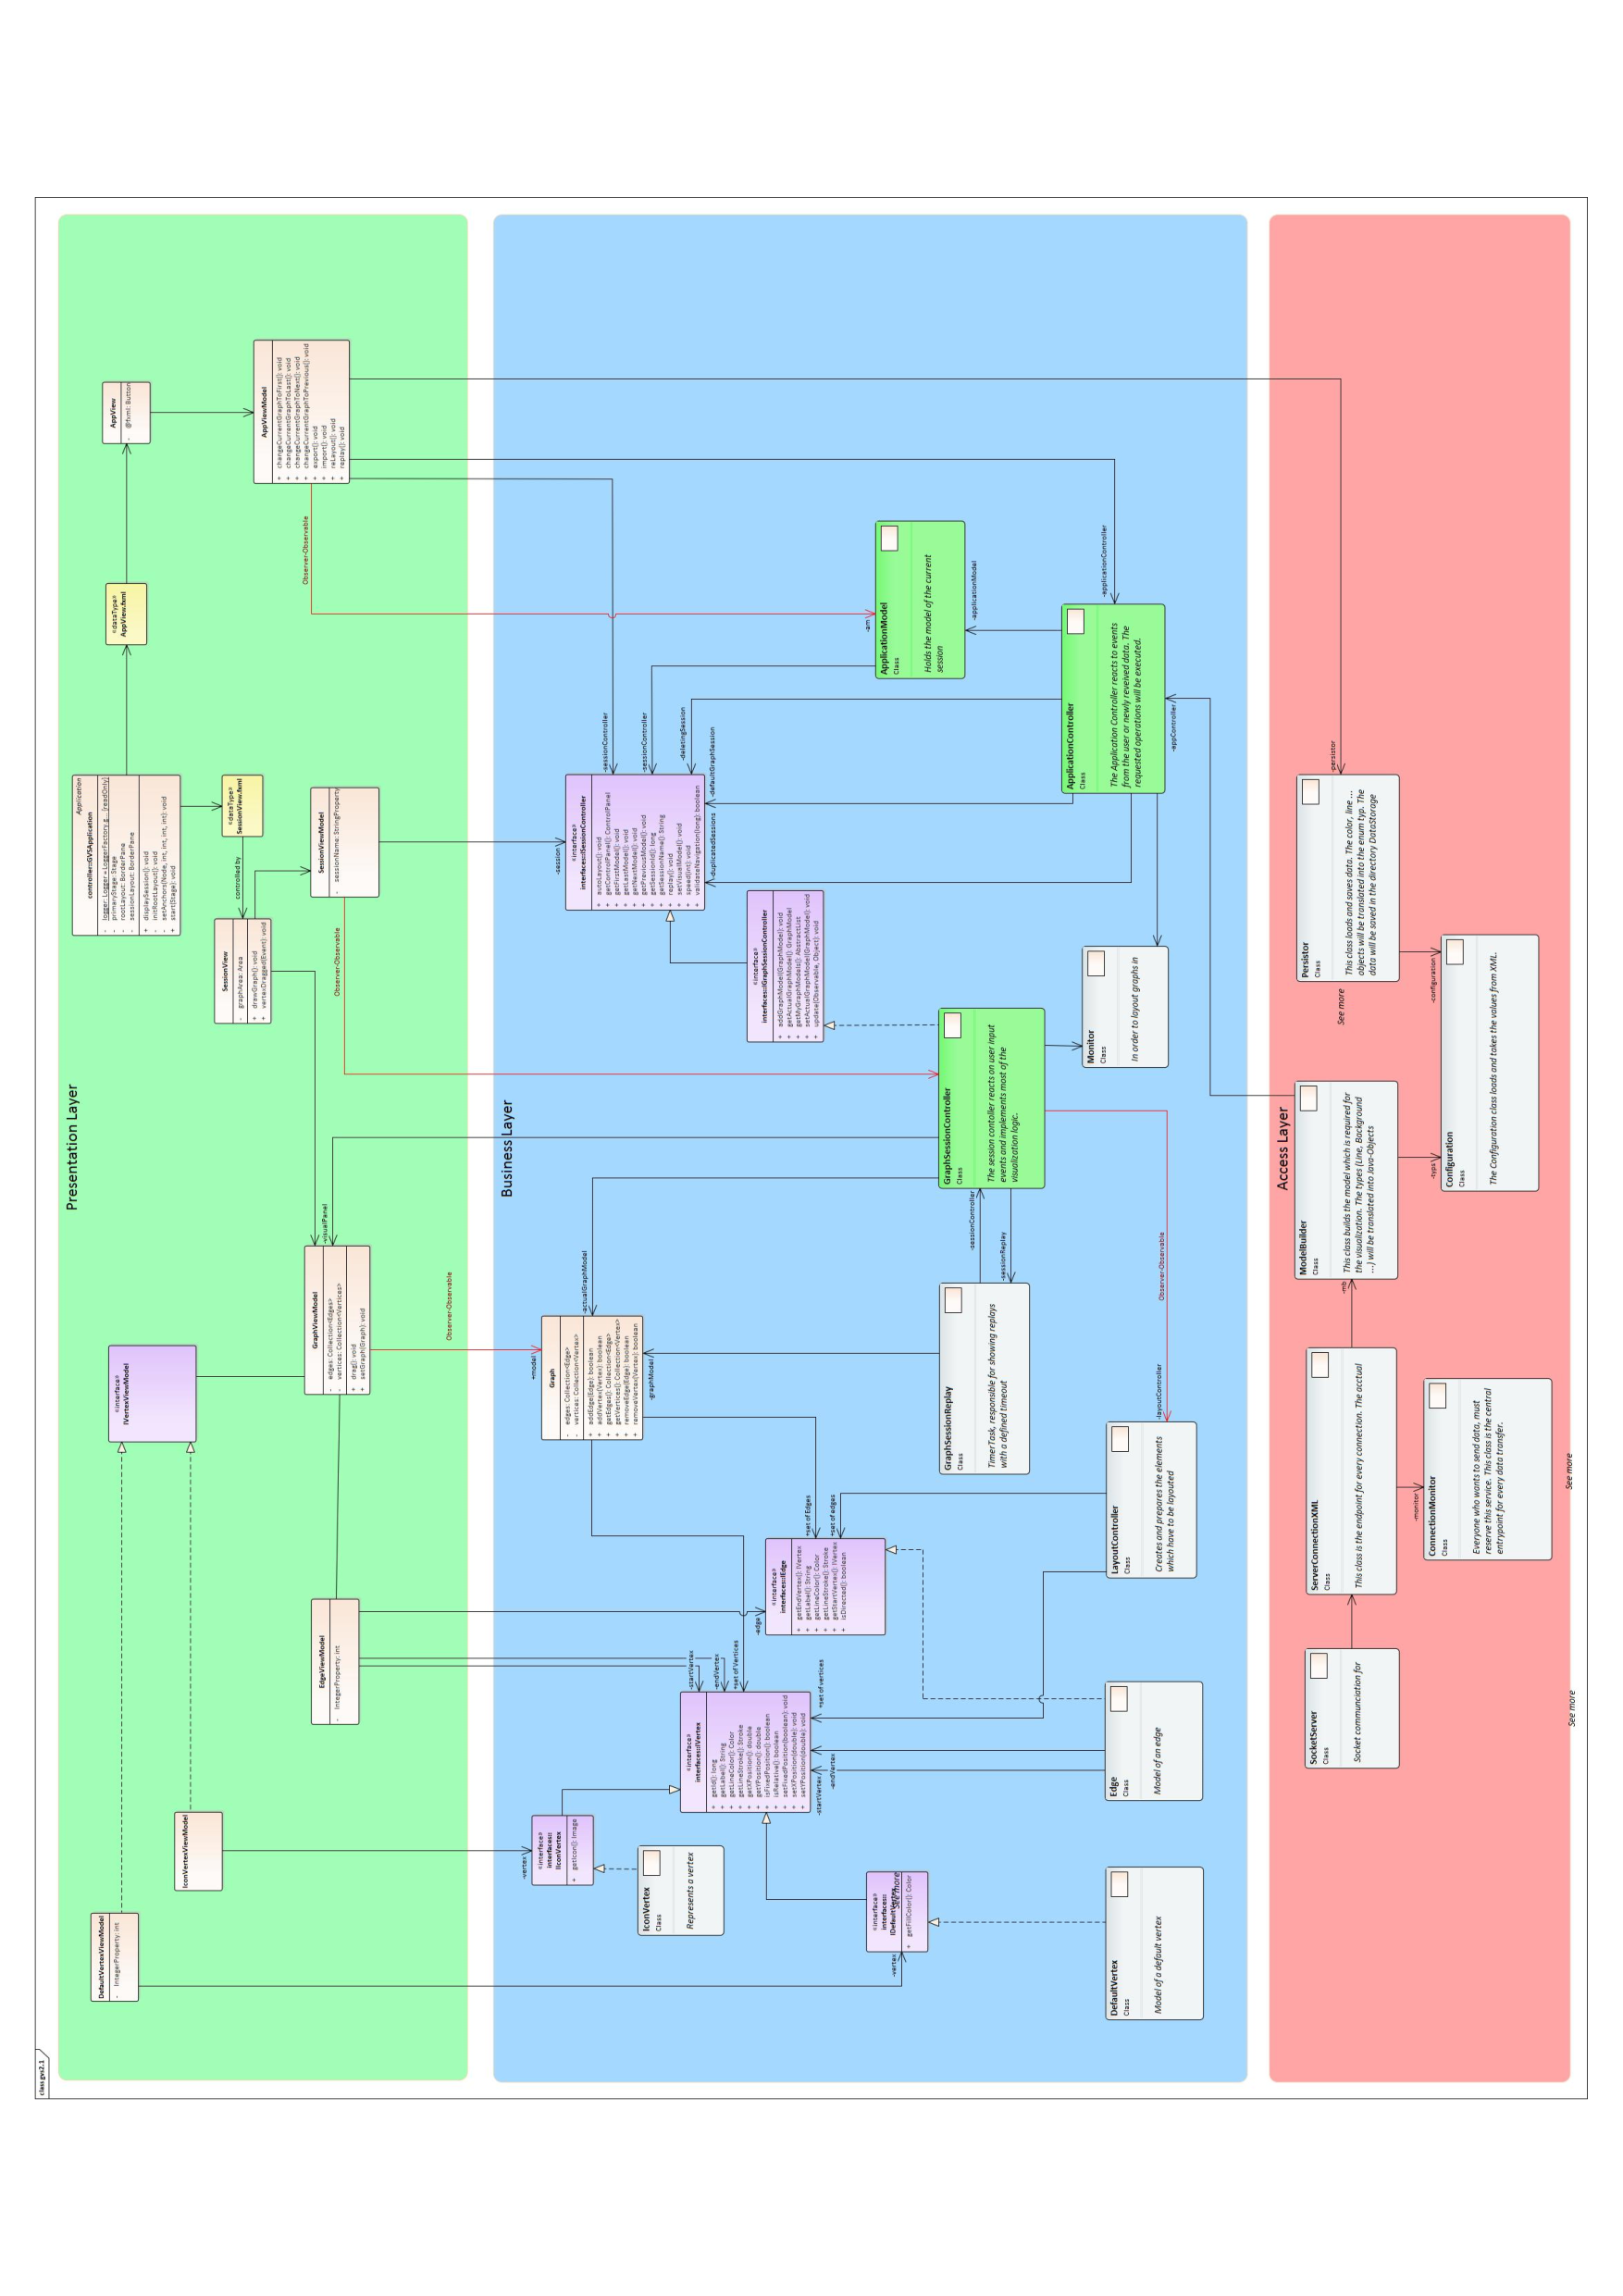
\includepdf[fitpaper]{assets/pdf/gvs2-1.pdf}
	
	\section{Schichtenstruktur} \label{ssec:layer-architecture}
	
	\subsection{Presentation Layer}
	Der Presentation Layer wurde von der restlichen Anwendung entkoppelt. Damit kann das eingesetzte UI Framework (z.B \gls{javafx}) leicht ersetzt werden. Der Presentation Layer ist nach dem \gls{mvvm} Prinzip organisiert.
	
	\subsubsection{Model-View-ViewModel} \label{sssec:mvvm}
	\gls{mvvm} dient der Trennung zwischen dem User Interface und der Anzeigelogik. \gls{mvvm} ist eine Konkretisierung des verbreiteten \gls{mvc} Pattern und setzt stark auf Databindings. Es wurde von Microsoft für das \gls{wpf} Framework entwickelt und wird auch in modernen \gls{javafx} Applikation eingesetzt.
	
	\begin{figure}[h!]
		\centering
		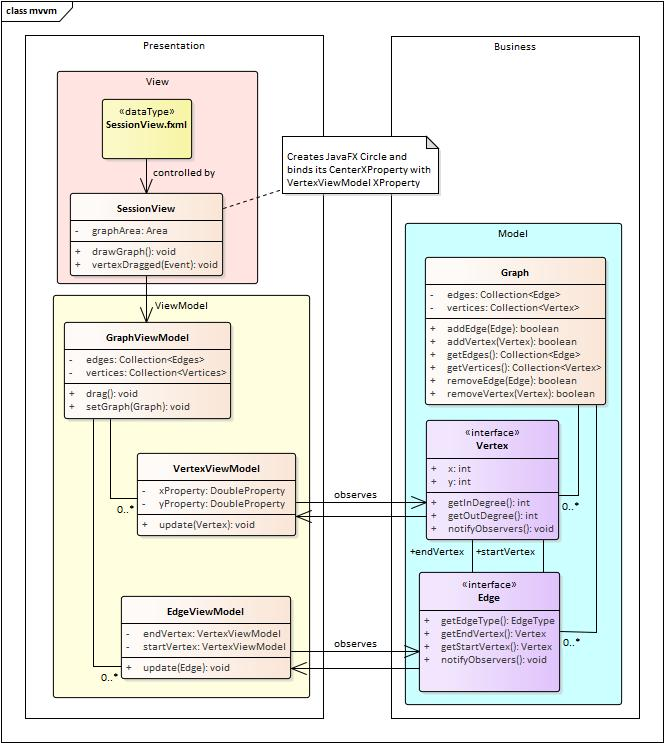
\includegraphics[width=0.7\linewidth]{assets/images/mvvm_concept}
		\caption[MVVM Konzept]{Mode View ViewModel Konzept}
		\label{fig:mvvmconcept}
	\end{figure}
	
	\paragraph{Model}
	Das \textit{Model} enthält reine Datenklassen ohne nennenswerte Logik. (siehe \gls{pojo}) Das \textit{Model} wurde in den Business Layer verschoben, damit das UI Framework einfach ausgewechselt werden kann. Werden die Werte im Model geändert, wird das \textit{ViewModel} über eine Observer Beziehung (\gls{observer}) benachrichtigt. Dies entspricht nicht dem klassischen \gls{mvvm} Konzept, wird jedoch benötigt, damit die View entsprechend aktualisiert wird, wenn z.B die Koordinaten neu berechnet werden.
	
	\paragraph{View}
	Die \textit{View} stellt den UI Zustand des \textit{ViewModels} dar. Sie setzt sich aus einer Controller Klasse sowie einer deklarativen \gls{fxml} Datei zusammen. Die View hält eine Instanz des ViewModels und leitet die eingehenden Anfragen direkt an dieses weiter. Mit der Databinding-API wird eine bidirektionale Kommunikation zwischen \textit{View} und \textit{ViewModel} sichergestellt. 
	
	\paragraph{ViewModel}
	Das \textit{ViewModel} kennt die View nicht. Es hat somit keine Abhängigkeiten zu konkreten Anzeige-Elementen. Dies hat den grossen Vorteil, dass die gesamte UI Logik im \textit{ViewModel} gekapselt ist und somit sehr gut testbar ist. Das ViewModel enthält \gls{javafx} spezifische Properties, die für das bidirektionale Binding zwischen UI Komponenten und Code Behind nötig sind.
	
	\subsection{Business Layer}
	Im Business Layer liegt die eigentliche Logik. Er enthält keine \gls{javafx} Komponenten, weshalb das eingesetzte UI Framework ohne weiteres ausgewechselt werden kann. 
	
	\subsection{Access Layer}
	Der Access Layer enthält Klassen für den Zugriff auf den Socket Server, sowie das File System. Es Ist für das Parsen von eingehenden XML Files zuständig und für deren Umwandlung in Domainobjekte.

	\section{Refactoring Konzept} \label{sec:refactroing-conpet}
	Im Rahmen dieser Studienarbeit soll die GVS 1.0 Applikation ein umfangreiches Refactoring erfahren. In diesem Unterkapitel wird beschrieben, wie dabei vorgegangen wird.
	
	\subsection{Ablauf}\label{ssec:ablauf}
	\begin{enumerate}
		\item Der Presentation Layer wird ersetzt. Dabei wird \gls{swing} durch \gls{javafx} ersetzt. Mehr Details finden sich in der Migrations Liste (\ref{ssec:class-refactroing-list}) sowie im Klassendiagramm von GVS 2.0 (\ref{sec:class-diagram})
		\item Die GVS 1.0 Library wird um Generics erweitert.
		\item Eine klare Schichtenarchitektur (\ref{ssec:layer-architecture}) wird eingeführt. Besonders wichtig ist dabei, die Entfernung von \gls{tangle}s.
		\item Duplicated Code und weitere Code Smells sollen entfernt werden. Ein besonderes Augenmerk wird auf ein konsequentes Naming, das DRY Konzept sowie das ''Single Responsibility'' Konzept für Klassen und Methoden gelegt.
	\end{enumerate}

	\subsection{Migrations Liste}
	\label{ssec:class-refactroing-list}
	Die folgende Liste soll zeigen, welche Klassen aus GVS 1.0 übernommen werden und welche Klassen in welcher Art und Weise verändert oder neu erstellt werden.
	
	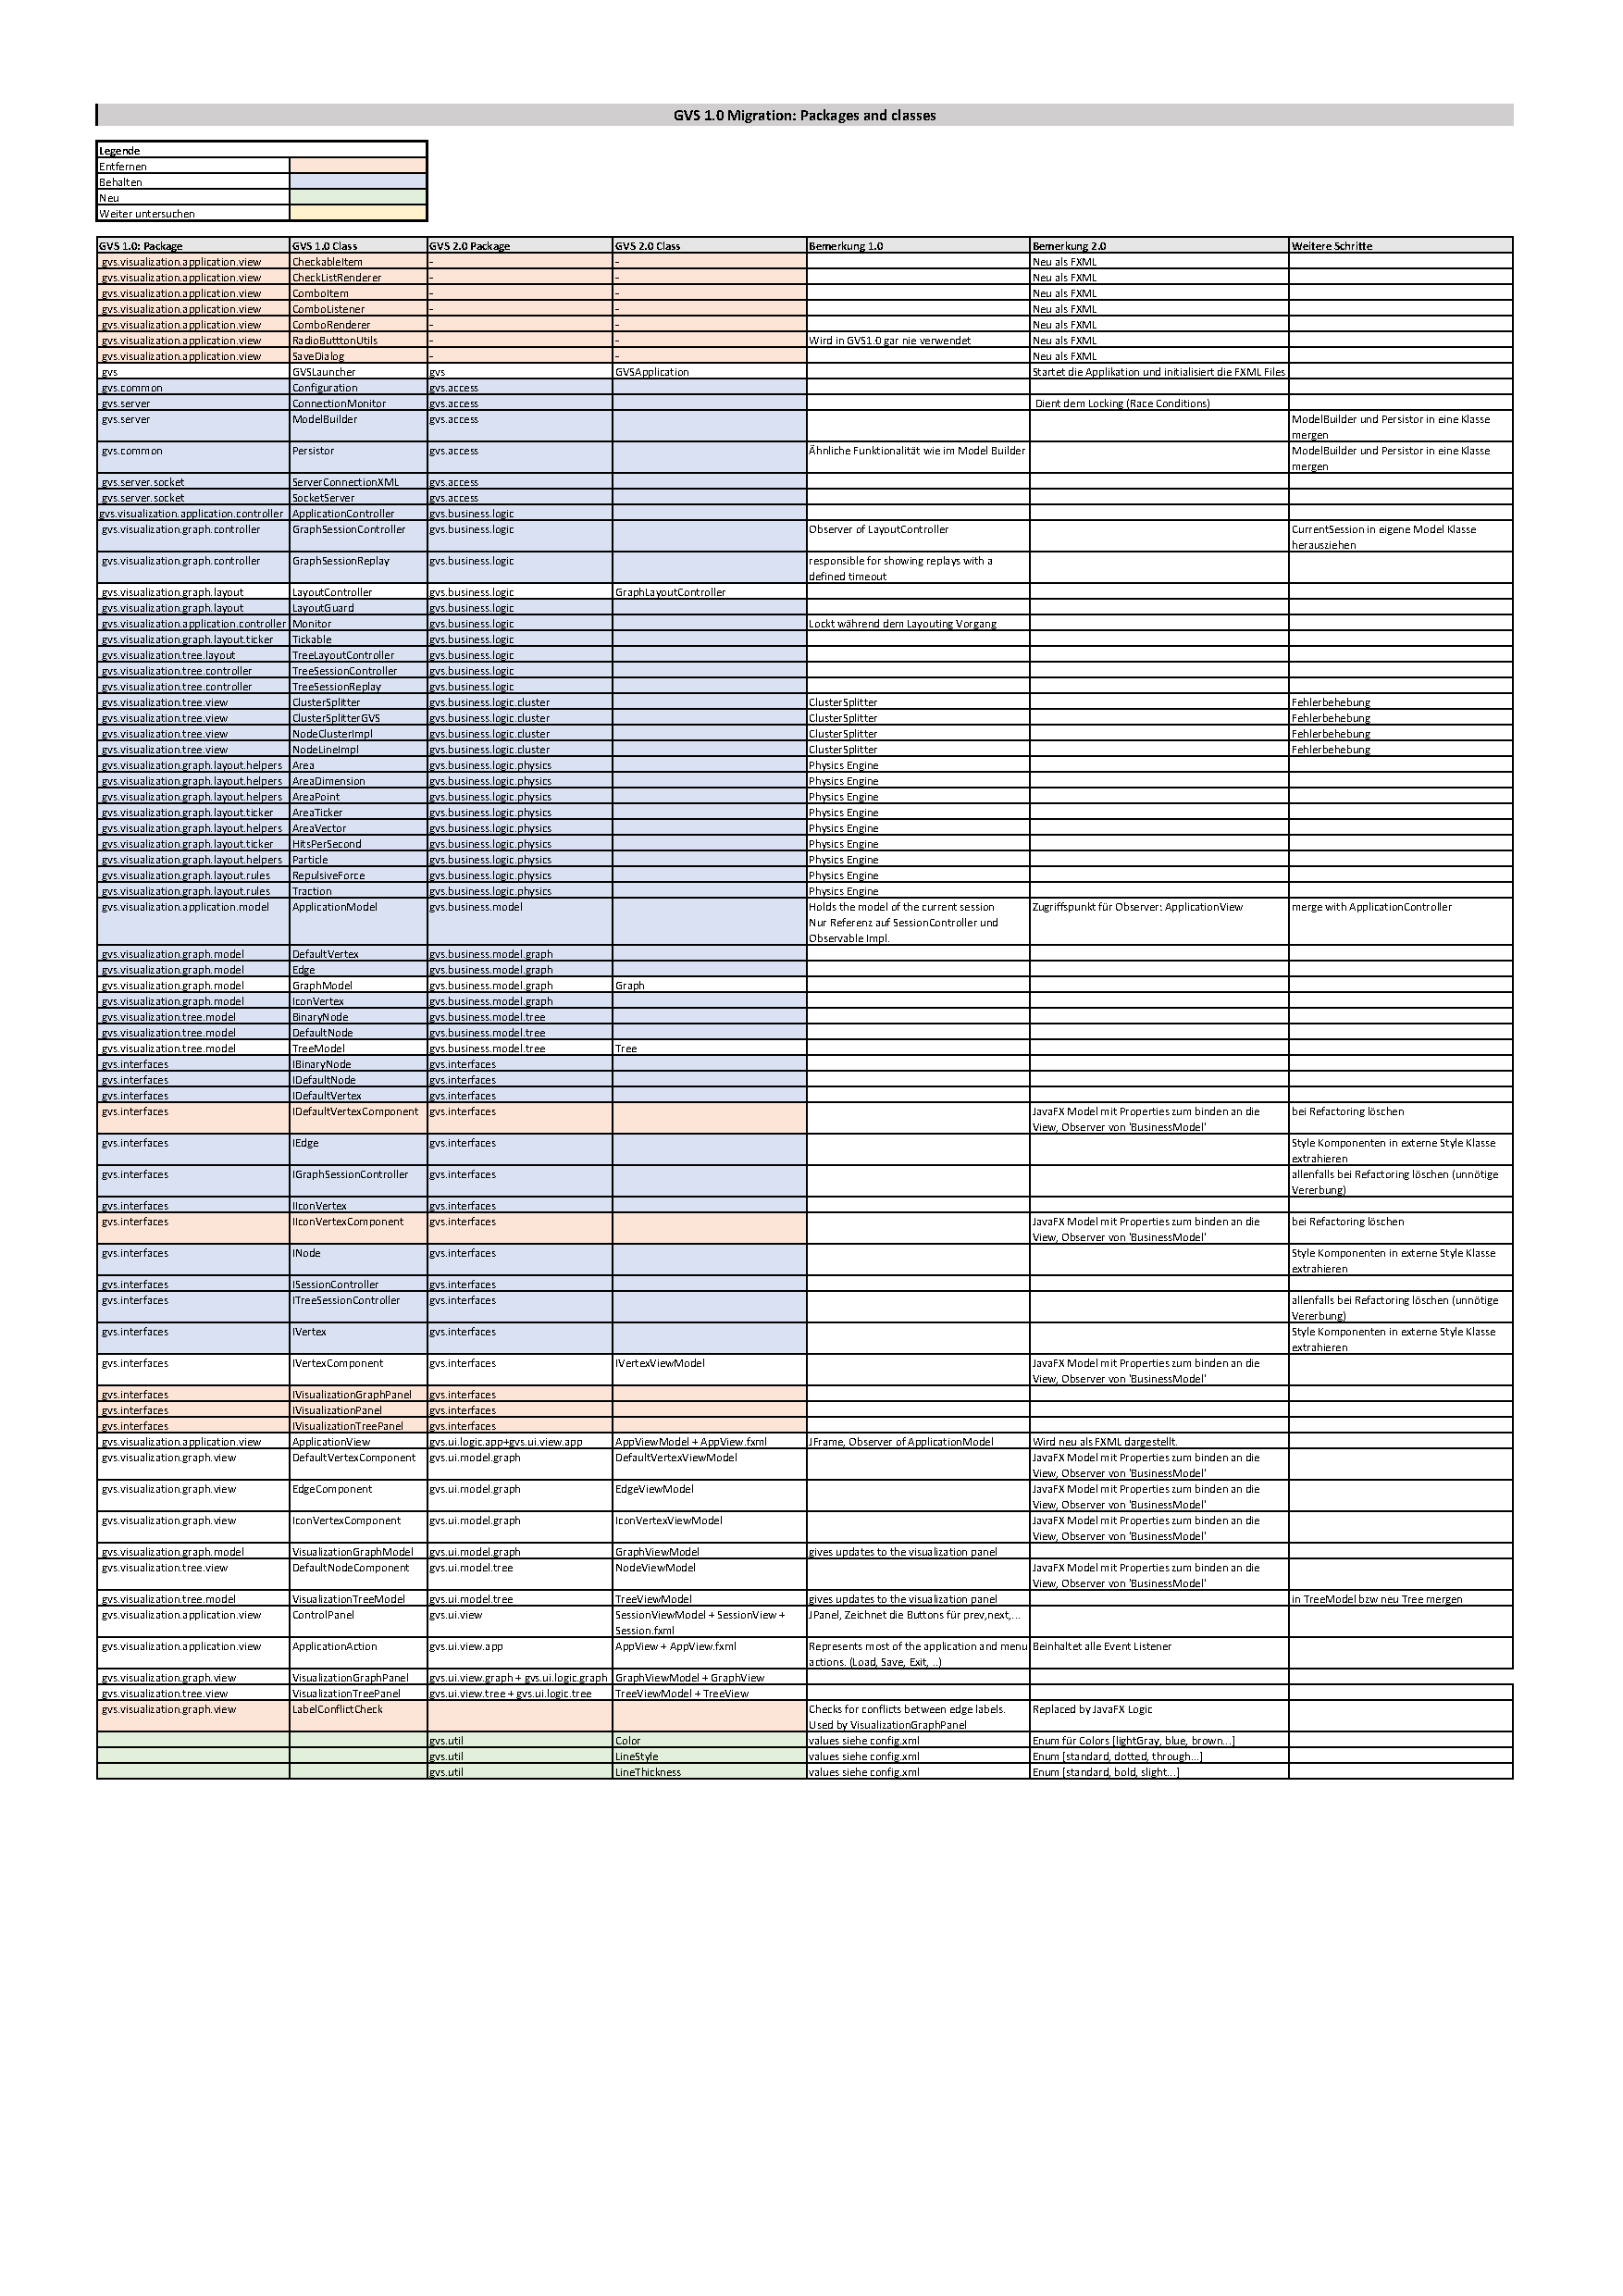
\includepdf[fitpaper]{assets/pdf/Migration_Replacements.pdf}
	
	\chapter{Realisierung}
		
	\begin{table}[h!]
	\centering
	\begin{tabularx}{\linewidth}{l l X l}
		\toprule 
		Datum & Version & Änderungen & Autor \\
		\midrule
		28.09.17 & 1.0 & Dokument erstellt & mwieland \\
		\bottomrule 
	\end{tabularx} 
	\caption{Versionshistory Realisierung} 
	\end{table}
	
	\section{UI Design}
	
	\subsection{FXML}
	
	\subsection{Logo}
	Das Logo wurde von den Eigenschaften des Kraken \cite{kraken} inspiriert. Kraken sind bekannt dafür, dass sie viele Irrgarten-Probleme effizient lösen können. Dies ist eine Anspielung an die Algorithmen, die vom \gls{gvs} unterstützt werden. Ebenfalls wurden die Saugnäpfe des Kraken als Graph visualisiert und auf der Stirn ist ein binärer Baum zu erkennen. 
	
	\begin{figure}[h!]
		\centering
		
\includegraphics[width=0.7\linewidth]{assets/images/logo}
		\caption[GVS Logo]{Graphs-Visualization-Service Logo}
		\label{fig:logo}
	\end{figure}
	
	
	\chapter{Ausblick}
	
	\section{Server Ausbau}
	
	\subsection{Threading Konzept}
	%TODO Multi or Single Threading?
	
	\section{Client Ausbau}
	
	\subsection{Algorithmen Library}
	
	\subsection{Annotations}
	
	
	
	\chapter{Projektmanagement}
	
	
	\begin{table}[h!]
		\centering
		\begin{tabularx}{\linewidth}{l l X l}
			\toprule 
			Datum & Version & Änderungen & Autor \\
			\midrule
			25.09.17 & 1.0 & Dokument erstellt & mwieland, mtrentini \\
			28.09.17 & 1.1 & Risikomanagement hinzugefügt & mtrentini \\
			03.10.17 & 1.2 & IDE, Frameworks, Buildprozess, Qualitätsmanagement hinzugefügt, & mwieland \\
			05.10.17 & 1.3 & Meilensteine definiert & mtrentini \\
			\bottomrule 
		\end{tabularx} 
		\caption{Versionshistory Projektmanagement} 
	\end{table}
	
	\section{Meilensteine}
	\label{sec:milestones}
	
	\subsubsection{Meilenstein 1: Analyse}
	Analyse des Ist-Zustandes von GVS 1.0: Die Problemdomäne wird spezifiziert. Mehrere Diagramme zeigen die Schnittstelle zwischen dem Business Layer und dem Presentation Layer auf. Es ist ersichtlich, wie die einzelnen Komponenten miteinander kommunizieren bzw. wie die Daten von der Socket ans UI weiter gereicht werden.
	
	\subsubsection{Meilenstein 2: Entwurf}
	\label{milestone2}
	Entwurf des Soll-Zustand von GVS 2.0: Eine klassische 3-Schichten Architektur wird entworfen. Es wird spezifiziert, welche GVS 1.0 Komponenten durch welche GVS 2.0 Komponenten ersetzt werden. Die in der Aufgabenstellung (\ref{aufgabenstellung}) geforderten Requirements werden festgehalten.
	
	\subsubsection{Meilenstein 3: Release 1}
	Der Presentation Layer ist vollständig gemäss Refactroing Konzept (\ref{sec:refactroing-conpet}) umgesetzt.
	
	\subsubsection{Meilenstein 4: Release 2}
	Die im Refactoring Konzept (\ref{sec:refactroing-conpet}) beschlossenen Änderungen sind umgesetzt. Das mit dem Enterprise Architekt erstellte Klassendiagramm ist mit dem Stand der GVS 2.0 Software synchron.
	
	\subsubsection{Meilenstein 5: Release 3}
	Alle im Meilenstein 2 definierten Requirements wurden umgesetzt. Die GVS 2.0 Software ist für den Einsatz im Unterricht bereit.
	
	\begin{table}[h!]
		\centering
		\begin{tabular}{l l l l}
			\toprule 
			\# & Name & Artefakte & Datum \\
			\toprule 
			1 & Analyse & Domainmodell & 18.10.17 \\
			& & Sequenzdiagramme & \\
			& &  Komponentendiagramm & \\
			\midrule
			2 & Entwurf  & Requirements & 25.10.17\\
			& & Schichtendiagramm & \\
			\midrule
			3 & Release 1 & GVS 2.0.1 & 15.11.2017 \\
			\midrule
			4 & Release 2 & GVS 2.0.2 & 06.12.2017 \\
			\midrule
			5 & Release 3 & GVS 2.0.3 & 22.12.2017 \\
			\bottomrule 
		\end{tabular} 
		\caption{Meilensteine} 
	\end{table}
	
	\subsection{Artefact Overview}
	Im Artefact Overview sind sämtliche zu erbringende Arbeitsergebnisse mit ihren Fertigstellungsdaten aufgelistet. Wenn nötig sind verschiedene Versionen gekennzeichnet.
	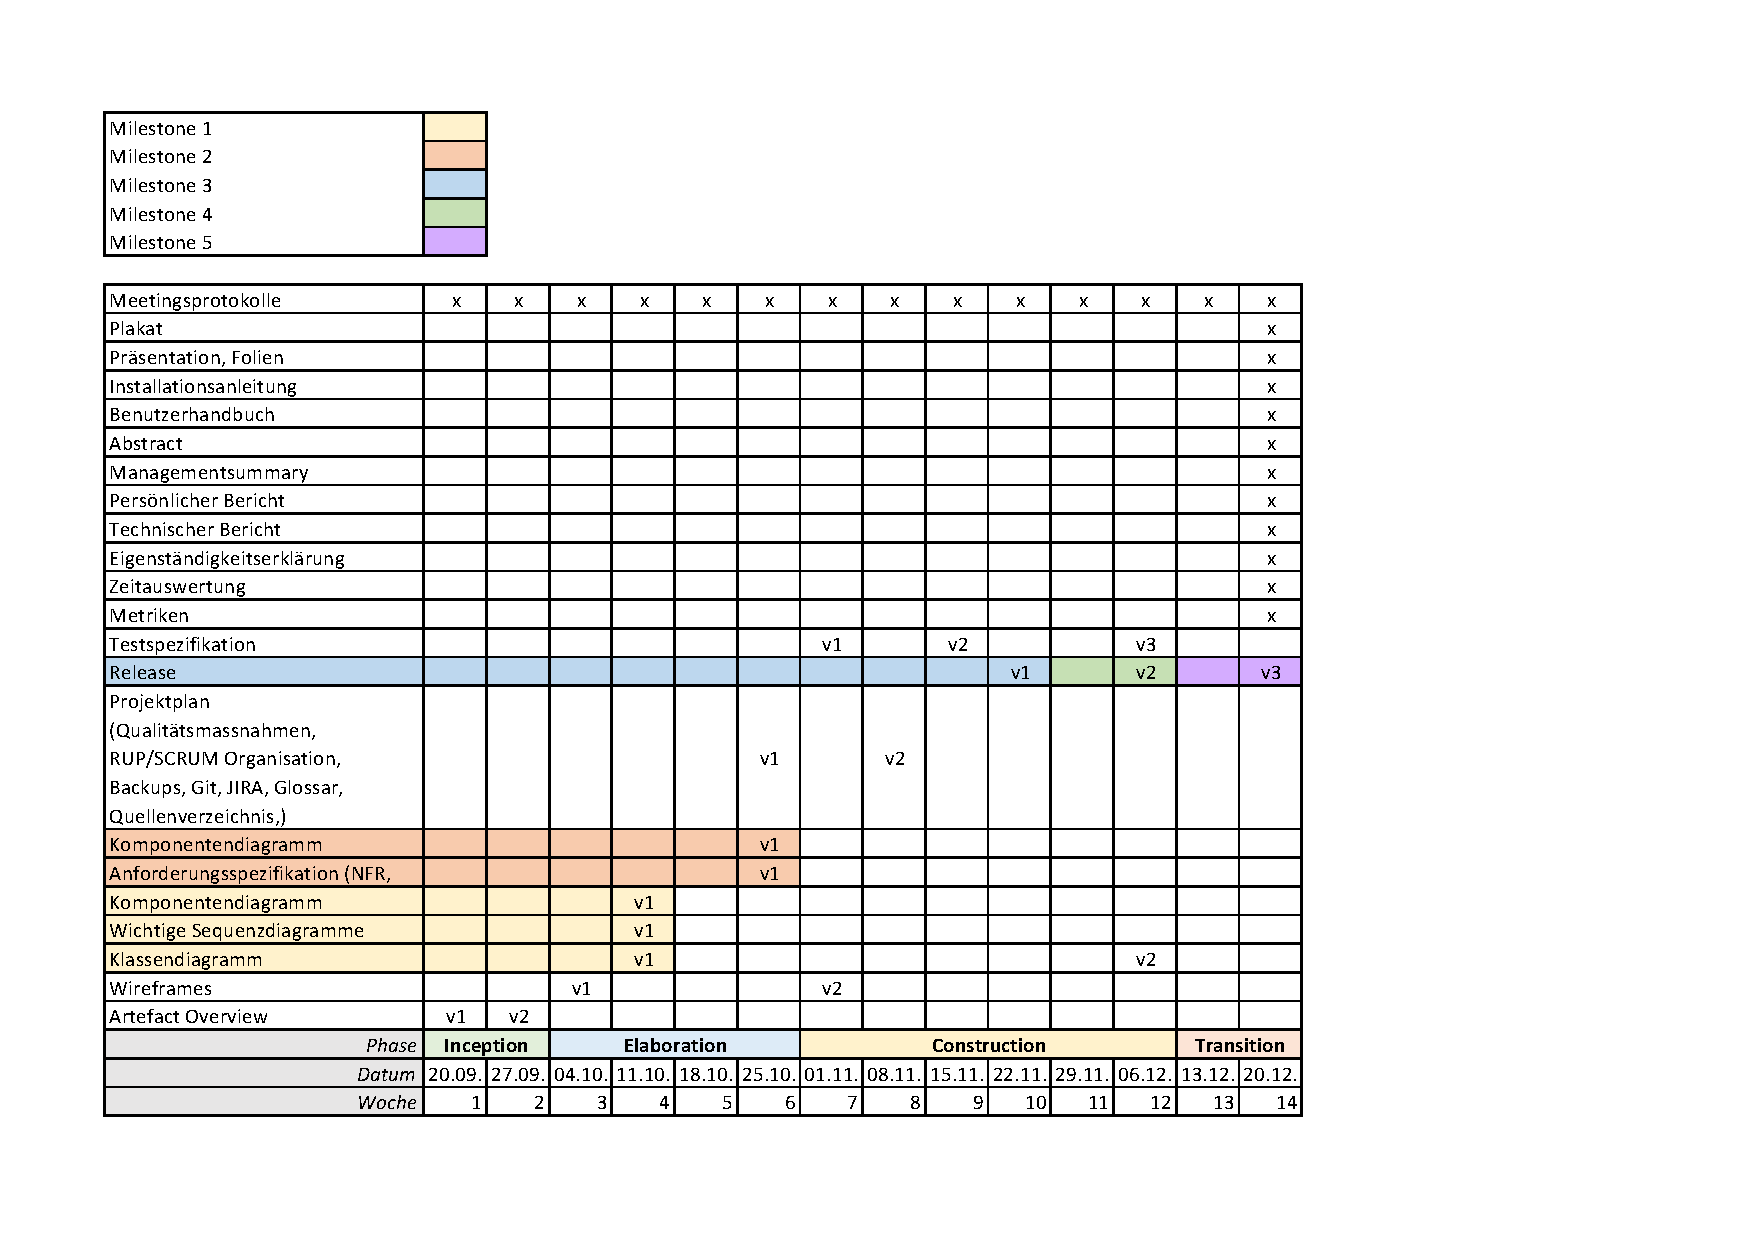
\includepdf[landscape]{assets/pdf/artefact_overview.pdf}
	
	\section{Zeitplanung}
	
	Das Projekt wird im Rahmen der Studienarbeit durchgeführt. Insgesamt stehen 14 Wochen zur Verfügung in welchen jedes Teammitglied 240 Stunden leisten muss. Somit entstehen ca. 17 Stunden Arbeitsaufwand pro Woche und Teammitglied.
		
	\section{Projektverwaltung}
	
	Als Projektmanagement Software wird Jira \cite{jira} eingesetzt. In Jira werden alle Requirements als Issues erfasst und in den Product Backlog eingepflegt. Pro Iteration sollen jeweils so viele Issues eingeplant werden, wie unter Berücksichtigung von administrativen Aufgaben abgearbeitet werden können. Dabei spielt der Teamspeed eine grosse Rolle, welcher sich über die Projektdauer einpendeln soll. 

	
	\subsection{Iterationsplanung}
	Die Iterationsplanung orientiert sich grob am \gls{rup} und ist unterteilt in eine Inception-, Elaboration-, Construction- sowie eine Transition-Phase. Jede Phase besteht aus einer oder mehreren Iterationen, die jeweils 1 Wochen dauern und am Freitag enden. Die Sprints sind bewusst nur 1 Woche lang, um eventuell ändernden Anforderungen gerecht zu werden. Zudem bringen die Wochenmeetings (\ref{ssec:meeting}) jeweils neuen Input, welcher dann direkt in den nächsten Sprint einfliessen kann.\\
	Eine Iteration wird nach \gls{scrum} organisiert. Am Anfang des Sprints definiert das Projektteam die zu erledigenden Issues und schätzt deren Aufwand. (Siehe \ref{sec:estimations}) Jeweils am Ende eines Sprints wird die geleistete Arbeit reflektiert. Entsprechende Erkenntnisse und Verbesserungen werden fortlaufend in die Projektorganisation aufgenommen. 
		
	\subsection{Schätzungen}
	\label{sec:estimations}
	Issues werden auf Basis von Story Points geschätzt. Dieses Vorgehen hat sich mit SCRUM etabliert. Die Nutzung von Story Points führt dazu, dass nicht die individuell unterschiedliche Bearbeitungszeit, sondern die Komplexität einer User Story geschätzt wird. Dies vereinfacht  und homogenisiert die Schätzungen und hilft den Teamspeed zu bestimmen.\cite{storypoints, storypoints2}
	
	\subsection{Zeitauswertung}
	Für die Zeitauswertung wird das Jira Plugin Tempo \cite{jiratempo} verwendet. Dieses bietet umfassende Auswertungsmöglichkeiten, sowie Exports nach MS Excel. Die Reports zur geleisteten Zeit befinden sich im Anhang \ref{zeitauswertung}.
	
	\subsection{Meetings} \label{ssec:meeting}
	Über die gesamte Projektdauer findet jeweils am Mittwoch um 17:15 ein wöchentliches Standortmeeting statt. Die Beschlüsse aus den Meetings werden protokolliert und bis spätestens 24h später an alle Teilnehmer versendet. Allfälliges Feedback wird nachträglich eingepflegt und versioniert abgelegt.
	
	\subsection{Branch Konzept}
	Die Branch Struktur orientiert sich an Gitflow \cite{gitflow}. Pro Issue wird ein Feature Branch erstellt, der nach erfolgreichem Review in den Development Branch gemerged wird. Beim Erreichen eines Meilensteins (siehe \ref{sec:milestones}) wird der Entwicklungszweig in den Master Branch gemerged.
	
	\section{Entwicklungsumgebung}
	Als \gls{ide} wird Eclipse mit folgenden Plugins verwendet
	\begin{itemize}
		\item FindBugs \cite{findbugs} zur statischen Code Analyse
		\item Cobertura \cite{cobertura} zur Überprüfung der Test Abdeckung
		\item Stan4J \cite{stan4j} zur Überprüfung von zyklischen Abhängigkeiten
		\item Checkstyle \cite{checkstyle} zur Überprüfung der Coding Richtlinien.
	\end{itemize}

	\section{Frameworks}
	%TODO any additional libraries? 
	Als UI Framework wird gemäss Aufgabenstellung \gls{javafx} eingesetzt (siehe Anhang \ref{aufgabenstellung}). \gls{javafx} gilt seit 2014 als Standardlösung für grafische Java Anwendungen.Es ist eine komplette Neuentwicklung und der offizielle Nachfolger vom \gls{awt} \cite{awt} und \gls{swing} \cite{swing}. 

	\section{Repositories}
	Die Artefakte werden in verschiedenen Repositories auf GitHub versioniert abgelegt. So gibt es für die Dokumentation, die Meetings-Protokolle und den Sourcecode jeweils ein eigenes Repository.

	\section{Continuous Integration}
	Die Software wird nach jedem Commit mit Travis CI \cite{travisci} gebuildet. Dies garantiert, dass sämtliche Qualitätsmassnahmen stets eingehalten werden. (Siehe \ref{sec:qualitymeasures})
	
	\subsection{Buildprozess}
	\label{sec:buildprocess}
	Zur Erstellung der Software Artefakte wird Gradle \cite{gradle} eingesetzt. Gradle verwaltet alle externen Software Abhängigkeiten. Zusätzlich wird die Software nur dann gebuilded, wenn alle Metriktools grünes Licht geben. Es resultiert ein ausführbares \gls{jar}.
		
	\section{Qualitätsmanagement}
	\label{sec:qualitymeasures}
	
	\subsection{Unit Tests}
	Zur Sicherung der Software Qualität sind gute Tests unerlässlich. Da jedoch ein grosser Teil des Business Layers von GVS 1.0 übernommen wird, ist es nicht realistisch, für sämtliche Klassen Unit Tests nachzureichen. Klassen die neu erstellt oder einem weitreichendem Refactroing unterzogen werden, sollen hinreichenden mit Tests abgedeckt sein. Der Schwerpunkt liegt dabei auf der Qualität und nicht auf einer möglichst hohen Testabdeckung.
	
	\subsection{Definition of Done}
	Source Code wird erst zum Review freigegeben, wenn folgende Kriterien erfüllt sind.
	\begin{itemize}
		\item Die \gls{ide} rsp. Build Tool zeigt keine Warnungen und Fehler
		\item Es gibt keinen auskommentierten Code
		\item Es existieren sinnvolle Unit und Integrationstests für das Feature
		\item Alle Metriken geben grünes Licht
		\item Das Issue wurde in Jira \cite{jira} zum Review vermerkt
	\end{itemize}
		
	\subsection{Review}
	Nach Abschluss eines Issues wird dieses in Form eines Pull-Request an den Teampartner zum Review übergeben. Durch das Vier-Augen-Prinzip kann die Qualität des Produktes hoch gehalten werden. Zusätzlich haben beide Teampartner stets den selben Wissensstand.
	
	\subsection{Metriken}
	\subsubsection{Code Style}
	Als Styleguide wird eine angepasste Version des Sun Styleguide verwendet \cite{suncheckstyle}. Damit dieser im Projekt durchgängig eingehalten wird, wurde das Checkstyle Plugin \cite{checkstyle} in den Buildprozess integriert. (Siehe \ref{sec:buildprocess})	
	
	\subsubsection{Code Climate}
	%TODO Check technical debt
	Zur Überwachung des Technical Debt und der Testabdeckung wird die Github App Code Climate \cite{codeclimate} eingesetzt.  

	\section{Risikomanagement}
	Nachfolgend sind die wichtigsten Risiken für diese Arbeit aufgelistet. Gewichtet werden die Risiken nach Eintrittswahrscheinlichkeit und Schadenshöhe. \cite{risikomanagement}
	
	\begin{table}[h!]
		\centering
		\begin{tabular}{l c c}
			\toprule 
			\# & Eintrittswahrscheinlichkeit (E) & Schadensschwere (S) \\
			\toprule 
			1 & gering & leicht  \\
			2 & mittel & mittelschwer \\
			3 & hoch & schwer \\
			\bottomrule 
		\end{tabular} 
		\caption{Legende Risiken} 
	\end{table}
	\begin{landscape}		
		\subsection{Mögliche Risiken}
			\begin{table}[h!]
			\centering
			\begin{tabularx}{\linewidth}{l X l l X X}
				\toprule 
				\# & Beschreibung & E & S & Prävention & Massnahmen bei Eintritt \\
				\toprule 
				1 & Verlust von Daten auf Grund von technischen Störungen oder Diebstahl von persönlichen Notebooks & 2 & 1 & Backups (siehe \ref{sec:backup}) & Durch die Massnahmen muss höchstens ein Datenverlust von 8h aufgearbeitet werden. \\
				\midrule
				2 & Die Schnittstelle zwischen Business Logik und Presentation Layer ist weitaus weniger wohldefiniert als ursprünglich angenommen. Der nötige Zeitaufwand übersteigt die Schätzung um ein Vielfaches & 2 & 2 & Gute Recherche und Einarbeit in GVS 1.0, genügend lange Elaboration Phase & Rücksprache mit Betreuer. Überprüfen des Projektscopes und allenfalls Anpassung des Scopes. \\
				\midrule
				3 & Funktionalitäten von GVS 1.0, welche mit Swing umgesetzt wurden, werden durch JavaFX nicht oder unzureichend unterstützt & 1 & 2 & Einlesen in JavaFX, Funktionalitäten GVS 1.0 abklären & Alternative zur bestehenden Umsetzung finden \\
				\midrule
				4 & Eingesetzte Frameworks, Libraries und Cloud Services harmonieren nicht wie angenommen & 2 & 2 & Auf einen Software Stack setzen, der beliebt und weit verbreitet ist. Dies reduziert das Risiko, dass der gegenseitige Support fehlt. & Alternativen für inkompatible Services finden \\  
				\midrule 
				5 & Der geplante Funktionsumfang von GVS 2.0 übersteigt das Zeitbudget, dass im Rahmen der Studienarbeit zur Verfügung steht & 2 & 3 & Endprodukt in Teilkomponenten aufteilen. Pro Komponente den zeitlichen Aufwand bewerten. Klare Definition, welche Artefakte zwingend umgesetzt werden müssen. & Frühzeitige Rücksprache mit dem Betreuer, wenn sich abzeichnet, dass eine Komponente mehr Arbeit in Anspruch nimmt. \\  
				\bottomrule 
			\end{tabularx} 
			\caption{mögliche Risiken} 
		\end{table}
    \end{landscape}

	\subsection{Backups}
		\label{sec:backup}
		Zur Minimierung von allfälligen Datenverlusten wird wie folgt vorgegangen:
	
	\begin{enumerate}
		\item Täglich automatisiertes Backup aller Projektdaten im JIRA \cite{jira} (Zeiterfassung, erstellte Issues, Jira Konfiguration)
		\item Die Projektdokumentation sowie der Programmcode wird in den vier Github Repositories der Github Organisation \cite{github} versioniert abgelegt. Für die Projektmitglieder gilt der Grundsatz ''Commit early and often''.
		\item Weitere Artefakte werden auf Dropbox \cite{dropbox} abgelegt und dort automatisch gesichert und versioniert.
	\end{enumerate}
	
	
	\newpage
	
	\appendix
	\noappendicestocpagenum
	\addappheadtotoc
	\appendixpage
	
	% Glossary
	\printglossary
	\glsaddall
	
	% List of references
	\printbibliography[heading=bibintoc]
	
	{
		\hypersetup{linkcolor=black}
		\listoffigures
	}
	
	{
		\hypersetup{linkcolor=black}
		\listoftables
	}
	
	
	
	\chapter{Eigenständigkeitserklärung}
	Der/Die Verfasser/in erklärt hiermit, dass er/sie die vorliegende Arbeit selbständig, ohne fremde Hilfe und ohne Benutzung anderer als die angegebenen Hilfsmittel angefertigt hat. Die aus fremden Quellen (einschliesslich elektronischer Quellen) direkt oder indirekt übernommenen Gedanken sind ausnahmslos als solche kenntlich gemacht. Durch Copyright geschützte Materialien wurden in dieser Arbeit nicht in unerlaubter Weise genutzt. Die Arbeit ist in gleicher oder ähnlicher Form oder auszugsweise im Rahmen einer anderen Prüfung noch nicht vorgelegt worden.\\[2cm]
	\dotbox{Ort, Datum} \hfill \dotbox{Unterschrift des/der Verfassers/in}
	\hfill \\[2cm]
	\dotbox{Ort, Datum} \hfill \dotbox{Unterschrift des/der Verfassers/in}
	
	\chapter{Vereinbarung}
	
	Mit dieser Vereinbarung werden die Rechte über die Verwendung und die Weiterentwicklung der Ergebnisse der Studienarbeit GVS von Muriele Trentini und Michael Wieland unter der Betreuung von Thomas Letsch geregelt.\\
	Die Urheberrechte stehen der Studentin / dem Student zu.\\
	Die Ergebnisse der Arbeit dürfen sowohl von der Studentin / dem Student wie von der HSR nach Abschluss der Arbeit verwendet und weiter entwickelt werden\\[2cm]
	\dotbox{Ort, Datum} \hfill \dotbox{Unterschrift des/der Verfassers/in}
	\hfill \\[2cm]
	\dotbox{Ort, Datum} \hfill \dotbox{Unterschrift des/der Verfassers/in}
	
	\chapter{Aufgabenstellung}
	\label{aufgabenstellung}
	Die folgenden Seiten enthalten die offizielle Aufgabenstellung dieser Studienarbeit.
	
    
\includepdf[pages={1-}]{assets/Aufgabenstellung_GVS2.pdf}


	\chapter{Persönliche Berichte}
	\label{erfahrungsberichte}
	
	\chapter{Zeitauswertung}
	\label{zeitauswertung}
	
	\chapter{Testspezifikation}
	
	\chapter{Meeting Protokolle}
	
	
	
\end{document}

